\documentclass{report}
\usepackage[utf8]{inputenc}
\usepackage[english]{babel}
\usepackage[hidelinks]{hyperref}
\usepackage{graphicx}
\usepackage{amsmath}
\usepackage{amssymb}
\usepackage{color}
\usepackage{pgfplots}
\usepackage{mathrsfs}
\usepackage{natbib}
\usepackage{xspace}
\usepackage{amsthm}
\usepackage{chngcntr}

\bibliographystyle{apalike}
\setcitestyle{authoryear,open={[},close={]}}

\graphicspath{ {./images/} }
\pgfplotsset{compat=1.16}
\usepgfplotslibrary{external}
\tikzexternalize[prefix=figures/]

\renewcommand\vec{\mathbf}
\renewcommand\cite{\citep}
\newcommand{\norm}[1]{\left\lVert#1\right\rVert}
\newcommand*{\tran}{^{\mkern-1.5mu\mathsf{T}}}
\newcommand*\elide{\textup{[\,\dots]}\xspace}
\newcommand{\todo}{{\color{red} \textbf{TODO} }}

\newcommand{\quickwordcount}[1]{%
  \immediate\write18{texcount -1 -sum -merge #1.tex > #1-words}%
  \input{#1-words}words%
}

\newtheorem{theorem}{Theorem}
\newtheorem{lemma}[theorem]{Lemma}
\newtheorem{corollary}{Corollary}[theorem]
\theoremstyle{definition}
\newtheorem{definition}{Definition}
\newtheorem{example}{Example}
\newtheorem*{remark}{Remark}

\counterwithout{footnote}{chapter}

\pgfdeclarelayer{pre main}
\begin{document}

\begin{titlepage}
    \centering
    
	{\scshape\LARGE Senior Honours Project\par}
	\vspace{0.25cm}
	{
\includegraphics[width=0.8\textwidth]{logo.png} \par}
    \vspace{0.25cm}
	{\huge\bfseries Freeing Neural Training Through Surfing\par}
	\vspace{0.5cm}
	
    \vfill
    {\large \textit{Georg Wölflein\\170011885} \par}
	{\large \textit{Supervisor: Dr. Mike Weir} \par}
    
    \vspace{0.5cm}

    {April 13, 2020\par}

    \vfill
    
    Word count: \quickwordcount{report}
\end{titlepage}

\chapter*{Abstract}
\todo

\chapter*{Declaration}
``I declare that the material submitted for assessment is my own work except where credit is explicitly given to others by citation or acknowledgement.
This work was performed during the current academic year except where otherwise stated.
The main text of this project report is \quickwordcount{report} long, including project specification and plan.
In submitting this project report to the University of St Andrews, I give permission for it to be made available for use in accordance with the regulations of the University Library. 
I also give permission for the title and abstract to be published and for copies of the report to be made and supplied at cost to any bona fide library or research worker, and to be made available on the World Wide Web.
I retain the copyright in this work.''

\vspace{0.5cm}

\textit{Georg Wölflein}

\tableofcontents

\chapter{Introduction}
\textit{Describe the problem you set out to solve and the
extent of your success in solving it. You should include
the aims and objectives of the project in order of
importance and try to outline key aspects of your
project for the reader to look for in the rest of your
report.}
\todo

\section{Context survey}
\subsection{Artificial neural networks}
\label{sec:context_anns}
The first mathematical model representing neurons in the human brain, so-called \textit{perceptons}, was formulated by \textcite{mcculloch1943} (see Section \ref{sec:ann}).
In 1958, the psychologist Frank Rosenblatt published the first percepton learning algorithm \cite{rosenblatt1958}, but this type of network lacked the ability to learn mappings that were not \textit{linearly separable}.
It was not until the 1980s with the introduction of the backpropagation algorithm capable of training networks with hidden layers, that neural networks experienced a substantial rise in popularity.

\paragraph{Backpropagation}
To this date, the backpropagation (BP) algorithm, attributed to \textcite{rumelhart1986}, remains the prominent method of training neural networks.
It involves computing the gradient of the loss function with respect to the weights and then using some gradient-based optimisation technique such as gradient descent to update the weights.
With the rise in popularity of deep neural networks, methods have been developed to increase the speed of converging to a minimum. 
The two main approaches are parallelising the computation and using adaptive learning rates like in the `Adam optimizer' \cite{kingma2014}.
It is well-established that BP, provided a suitable choice of hyperparameters, is guaranteed to converge to a local (but likely not global) minimum.
A common technique to subdue the effect of this issue is to run BP multiple times with different random initialisations.

\paragraph{Derivative-free optimisation}
The class of derivative-free optimisation (DFO) algorithms are optimisation techniques that attempt to find a global optimum, requiring only an objective function, but no gradient information.
One example of such an algorithm is simulated annealing (SA), proposed by \citeauthor{kirkpatrick1983}, that mimics the motion of atoms in the physical process of a slowly cooling material \cite*{kirkpatrick1983}.
Originally employed in discrete optimisation problems such as the combinatorial travelling salesman problem \cite{cerny1985}, it was later generalized and applied to problems with continuous domains \cite{belisle1993}.
However, in a comparative study of derivative-free optimisation algorithms, \citeauthor{rios2009} found that SA performed relatively poorly in comparison to more modern DFOs on general optimisation problems\footnote{It is important to note that \citeauthor{rios2009} did not assess DFOs for the purpose of neural network optimisation, but rather compared their performances on general convex and non-convex optimisation problems.} \cite*{rios2009}.

The concept of applying DFO as a means of training neural networks is not unique to this project.
In the 1990s, several training regimes for neural networks were proposed that did not rely on derivative calculations, employing variants of random and local search \cite{hirasawa1998,battiti1995}.
These approaches seemed to find better minima and did not get stuck in local minima as BP did. 
More recently, a particular random search approach was affirmed in outperforming BP in the context of deep neural networks for reinforcement learning, although a different family of DFO algorithms, so-called genetic algorithms were proposed as a superior alternative \cite{such2017}.

A very recent work presents a DFO technique for neural networks that uses a variant of local search belonging in the family of random search algorithms \cite{aly2019}.
This technique parallels the finding from other works that DFOs are often able to escape some\footnote{Guaranteed convergence to a global minimum in every scenario is not asserted, although the results indicate that the local minima are not as `poor'.} local minima and thus produce better training results; however, they require more iterations and computational resources than BP. 

\citeauthor{aly2019}, \citeauthor{such2017}, and similar works studied the performance of their respective DFO algorithms for training neural networks with a large parameter space (in the order of $10^6$ parameters) which, while providing valuable practical insight, made it impossible to examine the structure of the loss surface analytically in order to assess issues such as severely suboptimal local minima.

\paragraph{The local minimum problem}
The local minimum problem, which arises when an algorithm converges to a suboptimal local minimum with a comparatively high loss value, has been extensively studied as a phenomenon in optimisation problems.
However, with regards to neural networks, there seems to be differing opinions on the severity of this issue. 
One frequently cited article claims that ``In practice, poor local minima are rarely a problem with large networks'' \cite{lecun2015}.
This is underpinned in theory by other works which proved the nonexistence of suboptimal local minima, although they make varying assumptions on the structure of the underlying neural networks \cite{kawaguchi2016,nguyen2018,laurent2018}.
On the other hand, a recent article asserts that ``The apparent scarcity of poor local minima has lead practitioners to develop the intuition that bad local minima \elide are practically non-existent'' \cite{goldblum2019}.
Therefore, it can be said that the local minimum problem is still an active area of research.

The local minimum problems as it relates to neural training has been investigated extensively here in St Andrews. 
One particularly promising approach seems to be setting subgoals on the goal path.
However, setting these subgoals requires some finesse.
\textcite{lewis1999} show that simply employing a linear chain of subgoals (such as in \textcite{gorse1997}) does not suffice in reliably finding the global minimum, but instead a non-linear chain of subgoals is required.
A technique of setting and achieving subgoals that does not rely on BP has been explored in \textcite{weir2000}.

\subsection{Implementation tools}
In both acedemia and industry, Python is the de facto standard programming language for machine learning. 
A 2019 analysis on the world-leading software development platform \href{https://www.github.com/}{GitHub} found that Python is the most popular language for open source machine learning repositories \cite{elliott2019}.
Python is a simple yet versatile language that natively supports different programming paradigms (imperative, functional, object-oriented, and more).
It is often called an interpreted language\footnote{There is nuance associated with this statement, but Python certainly exhibits more traits of an interpreted than a compiled language.} because it is dynamically typed and performs automatic memory management (garbage collection) which generally facilitates shorter code than compiled languages such as C or Java, but also means that pure-Python implementations of data-intensive algorithms will usually not be as efficient.
One of the most fundamental packages, \href{https://numpy.org/}{NumPy}, implements very efficient array manipulation operations that, although specified in Python, are carried out at a lower level for performance.

NumPy is just one piece of Python's rich ecosystem of packages that are maintained by open-source contributers in the scientific and engineering community.
The two main frameworks for machine learning are \href{https://www.tensorflow.org/}{TensorFlow} by Google and \href{https://www.pytorch.org/}{PyTorch} by Facebook. 
At their core, both frameworks facilitate the computation of mathematical operations on tensors, offering support for hardware acceleration via \textit{graphics processing units} (GPUs) and providing parallelisation strategies for distributed computing which is especially potent in the context of machine learning where many operations fit the \textit{single instruction, multple data} (SIMD) pattern.
A TensorFlow program is specified as a directed \textit{computational graph} where nodes represent operations and edges represent their inputs and outputs (data tensors) \cite{tensorflow2015whitepaper}.
In the new TensorFlow 2, this graph does not need to be explicitly constructed anymore but is created on the fly which is known as \textit{eager execution}, thereby providing the user with a simpler API similar to NumPy.
The slightly younger PyTorch framework provided dynamic computation graphs and a NumPy-like interface since its initial release in 2016, and more recently added support for static computational graphs.
Hence the newest versions of both frameworks provide similar computational capabilities.
They also facilitate the automatic computation of gradients which is useful for training neural networks. 
TensorFlow is one of the most popular repositories on GitHub, and PyTorch's popularity is rapidly growing \cite{github2019}.

\href{https://keras.io/}{Keras} is a neural network library for Python which is conceived as a high-level interface rather than a framework. 
It provides implementations of, and abstractions over, common components of neural networks such as layers, optimisers, and activation functions.
TensorFlow 2 adopted Keras as part of its core library so that the abstractions provided by Keras can easily be used with the TensorFlow backend.

One should not overlook the concept of interactive notebooks made possible by Python's interpreted nature -- that is, mixing rich text (markdown), Python code, and its output. 
Not only does this allow the programmer to make changes to the code without having to rerun the program, but it also provides a means of presenting Python code in a more engaging way than just comments.
Any type of Python output, including data visualisations, can be presented in such notebooks which makes it attractive for machine learning.
These notebooks can be created using the \href{https://jupyter.org/}{Jupyter} package or even run online in the with services such as \href{https://colab.research.google.com/}{Google Colab}. 

\section{Requirements specification}
This project is primarily a research project, its main focus lies in contriving and investigating an example of the local minimum problem in neural networks and designing a technique that tackles this issue. 
Of auxillary importance is a software framework that should be developed to not only to compare different neural training techniques, but also to ensure that the main theoretical results obtained regarding the local minimum problem are reproducible.
During the course of this project, the initial objectives formulated in the DOER document evolved, especially as a better understanding of the theoretical aspect of neural surfing was attained.
The primary objectives are enumerated below in order of decreasing importance.
\begin{enumerate}
    \item Contrive a minimalist version of the stripe problem and show that it provides a strong basis for investigating and resolving the suboptimal local minimum problem for neural networks.
    \item Investigate goal-connecting paths for this problem and design a “neural surfer” that attempts to find such a goal-connecting path.
    \item Design a generic framework with a well-defined interface for implementing different gradient-based and derivative-free neural training algorithms and implement such algorithms.
    \item For this framework, implement a tool that facilitates the comparison of neural training algorithms on a given problem (dataset) by visualising arbitrary user-specified metrics (including weight and output trajectories) during training in real time.
\end{enumerate}
In addition, a secondary objective for this project was identified:
\begin{enumerate}
    \item Investigate how the neural surfer can be generalized to more complex problems.
\end{enumerate}

\section{Software engineering process}
\todo
\LaTeX
\section{Ethics}
There are no ethical considerations. 
All questions on the preliminary self-assessment form were answered with ``NO'' and hence no ethics form had to be completed.




\part{Theory}
\chapter{Neural network theory}
\section{Supervised learning}

\paragraph{Regression model}
In machine learning, a regression model $f$ is defined as a mathematical function of the form
\begin{equation}
    \label{eq:reg_model}
    f(\vec{x}) = \hat{y} = y + \epsilon
\end{equation}
that models the relationship between a $D$-dimensional feature vector $\vec{x} \in \mathbb{R}^D$ of independent (\textit{input}) variables and the dependent (\textit{output}) variable $y \in \mathbb{R}$. 
Given a particular $\vec{x}$, the model will produce a \textit{prediction} for $y$ which we denote $\hat{y}$.
Here, the additive error term $\epsilon$ represents the discrepancy between $y$ and $\hat{y}$.

\paragraph{Labelled dataset}
A dataset consists of $N$ tuples of the form $\langle \vec{x}_i, y_i\rangle$ for $i=1,\dots,N$.
For each feature vector $\vec{x}_i$ (a row vector), the corresponding $y_i$ represents the observed output, or \textit{label} \cite{burkov2019}.
We use the vector
\begin{equation}
    \vec{y} = \begin{bmatrix}
        y_1 & y_2 & \cdots & y_N
    \end{bmatrix}\tran
\end{equation}
to denote all the labelled outputs in the dataset, and the $N \times D$ matrix
\begin{equation}
    \label{eq:sup_learn_input_matrix}
    \vec{X} = \begin{bmatrix}
        \vec{x}_1 & \vec{x}_2 & \cdots & \vec{x}_N
    \end{bmatrix}\tran
\end{equation}
for representing the corresponding feature vectors.

\paragraph{Supervised learning}
A supervised learning algorithm for a regression task infers the function $f$ given in (\ref{eq:reg_model}) from a set of \textit{labelled training data} of the form explained previously. 
We use the vector
\begin{equation}
    \label{eq:sup_learn_prediction}
    \vec{\hat{y}} = \begin{bmatrix}
        \hat{y}_1 & \hat{y}_2 & \cdots & \hat{y}_N
    \end{bmatrix}\tran
\end{equation}
to denote the prediction that $f$ produces for each training sample.

\section{Artifical neural networks}
Artifical neural networks (ANNs) take inspiration from the human brain and can be regarded as a set of interconnected neurons. 
More formally, an ANN is a directed graph of $n$ neurons (referred to as \textit{nodes} or \textit{units}) with weighted edges (\textit{links}).
Each link connecting two units $i$ and $j$ is directed and associated with a real-valued weight $w_{i,j}$. 

A particular unit $i$'s \textit{excitation}, denoted ${ex}_i$, is calculated as the weighted sum
\begin{equation}
    {ex}_i = \sum_{j=1}^n{w_{j,i} a_j} + b_i
\end{equation}
where $a_j \in \mathbb{R}$ is another unit $j$'s \textit{activation} and $b_i \in \mathbb{R}$ is the $i$th unit's \textit{bias}.
Notice that if there exists no link between unit $i$ and a particular $j$ then simply $w_{i,j}=0$ and therefore $j$ will not contribute to $i$'s excitation. 

The unit $i$'s activation is its excitation applied to a non-linear \textit{activation function}, $g_i$. We have
\begin{equation}
    \label{eq:ann_activation}
    a_i = g_i\left({ex}_i\right) = g_i\left(\sum_{j=1}^n{w_{j,i} a_j} + b_i\right).
\end{equation}

\paragraph{Activation functions}
In its original form, \citeauthor{mcculloch1943} defined the neuron as having only binary activation \cite{mcculloch1943}. 
This means that in our model from (\ref{eq:ann_activation}), we would require $a_i \in \{0, 1\}$ and hence an activation function of the form $g_\text{thres}: \mathbb{R} \rightarrow \{0, 1\}$ which would be defined\footnote{In fact, \citeauthor{mcculloch1943} defined the activation to be zero when $x<\theta$ for a threshold parameter $\theta \in \mathbb{R}$ and one otherwise, but in our model the bias term $b_i$ acts as the threshold.} as
\begin{equation}
    \label{eq:thres_activation}
    g_\text{thres}(x) = \begin{cases} 
        0 & x < 0 \\
        1 & x \geq 0
    \end{cases}.
\end{equation}

Commonly used activation functions in modern neural networks include the sigmoid
\begin{equation}
    S(x) = \frac{1}{1 + e^{-x}}
\end{equation}
and the rectified linear unit (ReLU)
\begin{equation}
    g_\text{ReLU} = \begin{cases}
        0 & x < 0 \\
        x & x \geq 0
    \end{cases}.
\end{equation}

\begin{figure}
    \centering
    \begin{tikzpicture}
        \begin{axis}[
            x=0.75cm,
            y=3cm,
            axis lines=center,
            xlabel={$x$}, xlabel style={anchor=west},
            ylabel={$S(x)$}, ylabel style={anchor=south},
            ymin=0, ymax=1.2,
            xmin=-3.3, xmax=3.3,
            samples=100,
            xtick={-3,...,3},
            ytick={0, 0.5, 1},
            title style={at={(0.5,1)},anchor=south,yshift=15.0},
            title={Sigmoid}
        ]
            \addplot[black] {1 / (1 + exp(-x))};
        \end{axis}
    \end{tikzpicture}
    \vspace{.05\textwidth}
    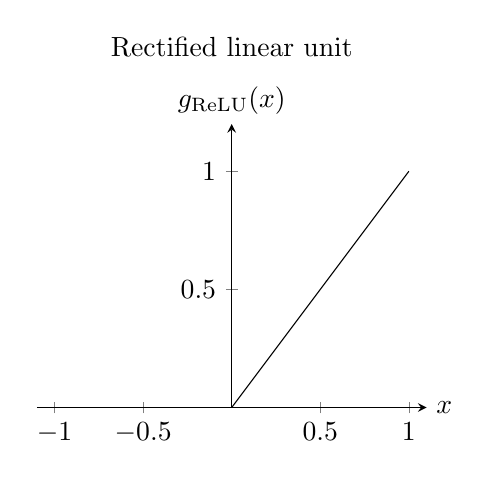
\begin{tikzpicture}
        \begin{axis}[
            x=2.25cm,
            y=3cm,
            axis lines=center,
            xlabel={$x$}, xlabel style={anchor=west},
            ylabel={$g_{\text{ReLU}}(x)$}, ylabel style={anchor=south},
            ymin=0, ymax=1.2,
            xmin=-1.1, xmax=1.1,
            samples=100,
            xtick={-1, -0.5, 0, 0.5, 1},
            ytick={0, 0.5, 1},
            title style={at={(0.5,1)},anchor=south,yshift=15.0},
            title={Rectified linear unit}
        ]
            \addplot[black][domain=0:1] {x};
            \addplot[black][domain=-1:0] {0};
        \end{axis}
    \end{tikzpicture}
    \caption{Plots of the the two most common activation functions.}
    \label{fig:activation_functions}
\end{figure}

Rectified units do not suffer from the \textit{vanishing gradient effect} \cite{glorot2011}.
This phenomenon occurs with sigmoid activation functions when they reach high saturation, i.e. when the input is significantly far from zero such that the gradient is almost horizontal.
However, the vanishing gradient problem is usually not prevelant in shallow\footnote{Shallow networks refer to ANNs with few layers.} networks so the sigmoid function still remains popular \cite{neal1992}.

\paragraph{ANNs as regression models}
We can employ an ANN to model a regression problem of the form given in (\ref{eq:reg_model}). 
To do so, we need at least $D+1$ neurons in the network. 
We consider the first $D$ units to be the \textit{input} neurons, and the last neuron, $n$, is the output unit.
Furthermore, we require $w_{j,k}=0$ for $j,k \in \mathbb{Z}^+$ where $j \leq n$ and $k \leq D$ to ensure that there are no links feeding into the input neurons.

To obtain the prediction $\hat{y}$ given the $D$-dimensional feature vector $\vec{x}$, we set the activation of the $i$th unit to the value the $i$th element in $\vec{x}$ for $i=1,\dots,D$.
Then, we propagate the activations using (\ref{eq:ann_activation}) until finally the prediction is the activation of the last neuron, $\hat{y}=a_n$.
This process is often called \textit{forward propagation} or \textit{forward pass} \cite{russell2010}.

\subsection{Single-layer network}
We introduce a single-layer network (SLN) as a type of ANN which consists of two conceptual layers, an input and an output layer.
Every input node is connected to every output node, but there are no intra-layer links (i.e. there are no links between any two input nodes or any two output nodes), as shown in Figure \ref{fig:single_layer_perceptron}. 
This is what we call a \textit{fully-connected feedforward} architecture.
SLN architectures will always form a \textit{directed acyclic graph} (DAG) because there are no intra-layer or backwards connections.

\begin{figure}
    \begin{center}
        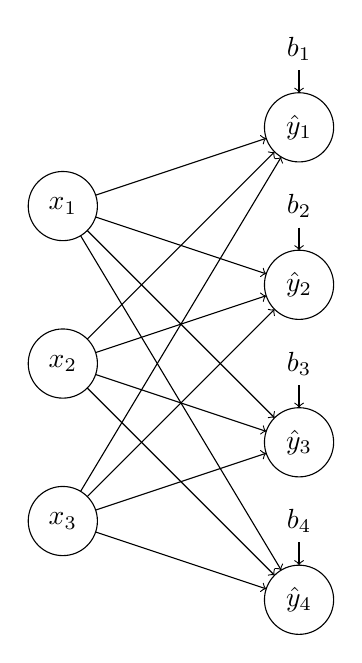
\begin{tikzpicture}
            [
                neuron/.style = {draw, circle, minimum size=25pt, inner sep=0pt, outer sep=0pt},
            ]
            \node [neuron] (x1) at (0,0) {$x_1$};
            \node [neuron] (x2) at (0,-2) {$x_2$};
            \node [neuron] (x3) at (0,-4) {$x_3$};
            \node [neuron] (n1) at (3,1)  {$\hat{y}_1$};
            \node [neuron] (n2) at (3,-1) {$\hat{y}_2$};
            \node [neuron] (n3) at (3,-3) {$\hat{y}_3$};
            \node [neuron] (n4) at (3,-5) {$\hat{y}_4$};
            \node (b1) at (3, 2) {$b_1$};
            \node (b2) at (3, 0) {$b_2$};
            \node (b3) at (3, -2) {$b_3$};
            \node (b4) at (3, -4) {$b_4$};
            \draw[->] (x1) -- (n1);
            \draw[->] (x1) -- (n2);
            \draw[->] (x1) -- (n3);
            \draw[->] (x1) -- (n4);
            \draw[->] (x2) -- (n1);
            \draw[->] (x2) -- (n2);
            \draw[->] (x2) -- (n3);
            \draw[->] (x2) -- (n4);
            \draw[->] (x3) -- (n1);
            \draw[->] (x3) -- (n2);
            \draw[->] (x3) -- (n3);
            \draw[->] (x3) -- (n4);
            \draw[->] (b1) -- (n1);
            \draw[->] (b2) -- (n2);
            \draw[->] (b3) -- (n3);
            \draw[->] (b4) -- (n4);
        \end{tikzpicture}
    \end{center}
    \caption{A single-layer perceptron with three input and four output neurons.}
    \label{fig:single_layer_perceptron}
\end{figure}

We purposefully use the term SLN instead of single-layer perceptron (SLP) to avoid confusion. 
A SLP has only one output unit and uses the threshold activation function given in (\ref{eq:thres_activation}) \cite{rosenblatt1958}.
In our definition of a SLN we allow more than one output and impose no restrictions on $g$, except that the same activation function is used for every output neuron.
We still use the term `single layer' because the input layer, lacking any incoming weight or bias connections, is not considered to be a `proper' layer.

Let us consider a SLN with $m$ inputs and $n$ outputs. 
Since every output unit $i$ only has connections from every input unit $j$,
we can adapt (\ref{eq:ann_activation}) to give the activation of a particular output neuron $i$ as
\begin{equation}
    a_i = y_i = g\left({ex}_i\right) = g\left(\sum_{j=1}^m{w_{j,i} x_j} + b_i\right)
    = g\left( \vec{w}_i\tran \vec{x}_i + b_i\right)
\end{equation}
where
$
    \vec{w}_i = \begin{bmatrix}
        w_{1,i} & w_{2,i} & \cdots & w_{m,i}
    \end{bmatrix}\tran
$
represents the weights of all the edges that connect to output unit $i$.
This is all we need to formally define a SLN.

\begin{definition}[Single-layer network]
    \label{def:sln}
    A SLN with $m$ inputs and $m$ outputs is the mathematical formula
    \begin{equation}
        \label{eq:single_layer_perceptron}
        \vec{f_{\text{SLN}}}(\vec{x}; \vec{W}, \vec{b}, \vec{g}) = \vec{g}\left( \vec{W}\tran \vec{x} + \vec{b} \right)
    \end{equation}
    where the  $m \times n$ matrix
    \begin{equation}
        \vec{W} = \begin{bmatrix}
            \vec{w}_1 & \vec{w}_2 & \cdots & \vec{w}_n
        \end{bmatrix} = \begin{bmatrix}
            w_{1,1} & w_{1,2} & \cdots & w_{1,n} \\
            w_{2,1} & w_{2,2} & \cdots & w_{2,n} \\
            \vdots & \vdots & \ddots & \vdots \\
            w_{m,1} & w_{m,2} & \cdots & w_{m,n}
        \end{bmatrix}
    \end{equation}
    captures all weights, the vector $\vec{b} = \begin{bmatrix}
        b_1 & b_2 & \cdots & b_n
    \end{bmatrix}\tran$ represents the biases, and $\vec{g}$ is the vector-valued activation function.
\end{definition}

Unlike the formula for a regression model, a SLN is a vector-valued function, due to the fact that there are multiple outputs. 
Note that when $n=1$, we reach the same form as in (\ref{eq:reg_model}). 
Moreover, if we additionally use the threshold activation function from (\ref{eq:thres_activation}), we arrive at the SLP model given by \citet{rosenblatt1958}.

\subsection{Multi-layer perceptron}
\label{sec:multi_layer_perceptron}
A multi-layer perceptron\footnote{Unlike SLPs, the activation function in a MLP as defined in literature does not necessarily need to be the binary threshold function $g_\text{thres}$; in fact, it is often one of the more modern activation functions explained in Section \ref{sec:activation_functions} \cite{hastie2017,burkov2019}. Hence we can use the term `multi-layer perceptron'.} (MLP) is a fully-connected feedforward ANN architecture with multiple layers which we will define in terms of multiple nested functions as in \citet{burkov2019}.
\begin{definition}[Multi-layer perceptron]
    \label{def:mlp}
    A MLP with $L$ layers is the mathematical function
    \begin{equation}
        f_{\text{MLP}}(\vec{x})
            = \hat{y}
            = f_L \left(
                \vec{f}_{L-1} \left(
                    \vec{\dots} \left(
                        \vec{f}_1 \left(
                            \vec{x}
                        \right)
                    \right)
                \right)
            \right)
    \end{equation}
    where $\vec{f}_l(\vec{x}) = \vec{f_{\text{SLN}}}(\vec{x}; \vec{W}_l, \vec{b}_l, \vec{g}_l)$ for $l = 1, \dots, L-1$. 
    The outermost function $f_L$ represents a SLN with only one output unit and is hence the scalar-valued function $f_L(\vec{x}) = f_{\text{SLN}}(\vec{x}; \vec{W}_L, \vec{b}_L, \vec{g}_L)$.
    This means that we can fully define the parameters of a MLP with the three-tuple
    \begin{equation}
        \label{eq:mlp_three_tuple}
        \langle \mathscr{W}, \mathscr{B}, \mathscr{G} \rangle
    \end{equation}
    where $\mathscr{W} = \vec{W}_1, \vec{W}_2, \dots, \vec{W}_L$ are the weight matrices, $\mathscr{B} = \vec{b}_1, \vec{b}_2, \dots, \vec{b}_L$ the bias vectors, and $\mathscr{G} = \vec{g}_1, \vec{g}_2, \dots, \vec{g}_L$ the vector-valued activation functions.
\end{definition}

Notice that for every $l < L$, $\vec{W}_l$ is a $n_l \times m_l$ matrix such that $n_l=m_{l+1}$ to esnure that the number of outputs of layer $l$ is the number of inputs to layer $l+1$.
This means that the MLP has $m_1$ input neurons.
Since the final layer has only one output unit, $\vec{W}_L$ has only one row, and finally $n_L=1$

The graph representing this type of network consists of connecting the outputs of the SLN representing layer $l$ with the inputs of the SLN representing layer $l+1$, as shown in Figure \ref{fig:multi_layer_perceptron}. 
The layers between the input and output layers are referred to as \textit{hidden} layers.

\begin{figure}
    \begin{center}
        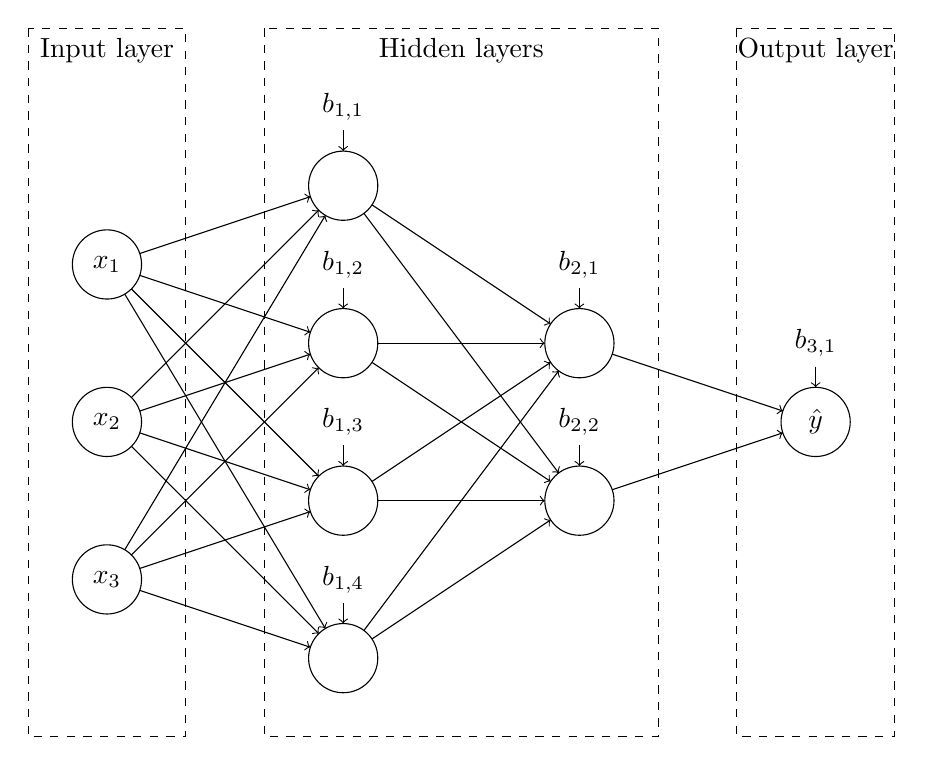
\begin{tikzpicture}
            [
                neuron/.style = {draw, circle, minimum size=25pt, inner sep=0pt, outer sep=0pt},
            ]
            \node [neuron] (x1) at (0,0) {$x_1$};
            \node [neuron] (x2) at (0,-2) {$x_2$};
            \node [neuron] (x3) at (0,-4) {$x_3$};
            \node [neuron] (h11) at (3,1) {};
            \node [neuron] (h12) at (3,-1) {};
            \node [neuron] (h13) at (3,-3) {};
            \node [neuron] (h14) at (3,-5) {};
            \node [neuron] (h21) at (6,-1) {};
            \node [neuron] (h22) at (6,-3) {};
            \node [neuron] (y) at (9, -2) {$\hat{y}$};
            \node (b11) at (3, 2) {$b_{1,1}$};
            \node (b12) at (3, 0) {$b_{1,2}$};
            \node (b13) at (3, -2) {$b_{1,3}$};
            \node (b14) at (3, -4) {$b_{1,4}$};
            \node (b21) at (6, 0) {$b_{2,1}$};
            \node (b22) at (6, -2) {$b_{2,2}$};
            \node (b3) at (9, -1) {$b_{3,1}$};
            \draw[->] (x1) -- (h11);
            \draw[->] (x1) -- (h12);
            \draw[->] (x1) -- (h13);
            \draw[->] (x1) -- (h14);
            \draw[->] (x2) -- (h11);
            \draw[->] (x2) -- (h12);
            \draw[->] (x2) -- (h13);
            \draw[->] (x2) -- (h14);
            \draw[->] (x3) -- (h11);
            \draw[->] (x3) -- (h12);
            \draw[->] (x3) -- (h13);
            \draw[->] (x3) -- (h14);
            \draw[->] (h11) -- (h21);
            \draw[->] (h11) -- (h22);
            \draw[->] (h12) -- (h21);
            \draw[->] (h12) -- (h22);
            \draw[->] (h13) -- (h21);
            \draw[->] (h13) -- (h22);
            \draw[->] (h14) -- (h21);
            \draw[->] (h14) -- (h22);
            \draw[->] (b11) -- (h11);
            \draw[->] (b12) -- (h12);
            \draw[->] (b13) -- (h13);
            \draw[->] (b14) -- (h14);
            \draw[->] (b21) -- (h21);
            \draw[->] (b22) -- (h22);
            \draw[->] (b3) -- (y);
            \draw[->] (h21) -- (y);
            \draw[->] (h22) -- (y);
            \draw[dashed] (-1,3) rectangle (1,-6);
            \draw[dashed] (2,3) rectangle (7,-6);
            \draw[dashed] (8,3) rectangle (10,-6);
            \node[below] (input) at (0,3) {Input layer};
            \node[below] (hidden) at (4.5,3) {Hidden layers};
            \node[below] (output) at (9,3) {Output layer};
        \end{tikzpicture}
    \end{center}
    \caption{A multi-layer perceptron with three inputs and two hidden layers.}
    \label{fig:multi_layer_perceptron}
\end{figure}

Since MLPs are simply nested SLNs, it follows that MLPs retain the DAG property and are therefore \textit{feedforward} networks as well.
In the forward pass, the activations are propagated from layer to layer (i.e. nested function to nested function) as in (\ref{eq:single_layer_perceptron}).



\chapter{Neural network learning}
\section{Gradient descent with mean squared error}
\section{Local minimum problem}
\section{Simulated annealing}

\chapter{Neural surfing theory}
\section{Weight and output spaces}
In Definition \ref{def:mlp} we established that the three-tuple from (\ref{eq:mlp_three_tuple}) is sufficient to fully define a MLP. 
Most importantly, we have $\mathscr{W} = \vec{W}_1, \vec{W}_2, \dots, \vec{W}_L$ and $\mathscr{B} = \vec{b}_1, \vec{b}_2, \dots, \vec{b}_L$ representing each layer's weight matrices and bias vectors, respectively. 

\begin{definition}[Weight space]
    We define the weight space $\mathcal{W}$ of a MLP as the set of all possible assignments to its \textit{trainable parameters}. 
    The trainable parameters are its weights and biases, so the weight space encompasses all possible configurations of $\mathscr{W}$ and $\mathscr{B}$. 
    Hence the weight space for a network with $P$ trainable parameters is defined as
    \begin{equation}
        \mathcal{W} = \mathbb{R}^P.
    \end{equation}
\end{definition}

\begin{lemma}
    A MLP with $L$ layers where the number of inputs to layer $l$ is given as $m_l$ will have a total of
    $P = \sum_{l=1}^{L-1}{\left(m_{l+1} (m_l + 1)\right)} + m_L + 1$
    trainable parameters.
\end{lemma}

\begin{proof}
    A SLN with $m$ inputs and $n$ outputs will have $m \times n$ weights and $n$ biases, totalling $n(m+1)$ trainable parameters.
    Now consider a MLP with $L$ layers, where $m_1, m_2, \dots, m_L$ is the number of inputs to each layer. 
    For any layer $l$, the number of outputs $n_l=m_{l+1}$ except for the last layer where $n_L=1$.
    It follows that the total number of trainable parameters in the network is
    \begin{align*}
        P &= \sum_{l=1}^{L}{\left(n_l (m_l + 1)\right)} \\
        &= \sum_{l=1}^{L-1}{\left(n_l (m_l + 1)\right)} + n_L (m_L + 1)\\
        &= \sum_{l=1}^{L-1}{\left(m_{l+1} (m_l + 1)\right)} + m_L + 1.
    \end{align*}
\end{proof}

\begin{definition}[Output space]
    The output space $\mathcal{O}$ spans the space of all possible output predictions on the training set.
    In Definition \ref{def:mlp}, it states that the network must only have one output node and thus the prediction $\hat{y}$ is a scalar. 
    From (\ref{eq:sup_learn_prediction}), the vector $\vec{\hat{y}}$ represents the prediction $\hat{y}$ for all $N$ training samples.
    This means that the output space spans all possible assignments of $\vec{\hat{y}}$, so
    \begin{equation}
        \mathcal{O}=\mathbb{R}^N.
    \end{equation}
\end{definition}

\begin{theorem}[Relationship between $\mathcal{W}$ and $\mathcal{O}$]
    For any SLN with one output unit, the function $h: \mathcal{W} \rightarrow \mathcal{O}$ mapping the weights to outputs is not a linear mapping.
\end{theorem}
\begin{proof}
    Let us consider a SLN with $m$ inputs and one output, as depicted in Figure \ref{fig:sln_m_in_1_out}.
    \begin{figure}
        \begin{center}
            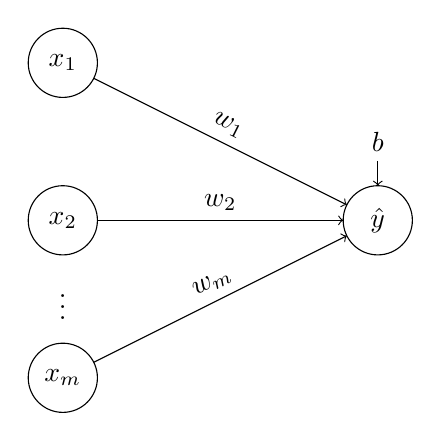
\begin{tikzpicture}
                [
                    neuron/.style = {draw, circle, minimum size=25pt, inner sep=0pt, outer sep=0pt},
                ]
                
                \node [neuron] (x1)  at (0,0) {$x_1$};
                \node [neuron] (x2) at (0,-2) {$x_2$};
                \node (dots) at (0,-3) {$\vdots$};
                \node [neuron] (xm) at (0,-4) {$x_m$};
                \node [neuron] (y) at (4,-2) {$\hat{y}$};
                \node (b) at (4, -1) {$b$};
                \draw[->] (x1) -- (y) node[midway, above, sloped] {$w_1$};
                \draw[->] (x2) -- (y) node[midway, above, sloped] {$w_2$};
                \draw[->] (xm) -- (y) node[midway, above, sloped] {$w_m$};
                \draw[->] (b) -- (y);
            \end{tikzpicture}
        \end{center}
        \caption{The DAG representing a SLN with $m$ inputs and one output unit.}
        \label{fig:sln_m_in_1_out}
    \end{figure}
    Modifying the formula for a SLN given in Definition \ref{def:sln} (\ref{eq:single_layer_perceptron}) for the case where there is only one output unit, we obtain
    $\hat{y} = f_\text{SLP}(\vec{x}; \vec{w}\tran, b, g) = g\left(\vec{w}\tran \vec{x} + b\right)$
    where
    $\vec{x} = \begin{bmatrix}
        x_1 & x_2 & \cdots & x_m
    \end{bmatrix}\tran$
    is the input feature vector.

    We will consider a dataset with $N$ samples where the input is given by a $N\times m$ matrix
    $\vec{X} = \begin{bmatrix}
        \vec{x}_1 & \vec{x}_2 & \cdots & \vec{x}_N
    \end{bmatrix}\tran$
    as in (\ref{eq:sup_learn_input_matrix}) and the labelled outputs $\vec{\hat{y}}$ are defined as in (\ref{eq:sup_learn_prediction}).
    For our SLN, the function $h: \mathcal{W} \rightarrow \mathcal{O}$ is defined as applying the SLN to each input sample, so
    \begin{equation*}
        h \left( \vec{w} \right)
        = \vec{\hat{y}}
        = \begin{bmatrix}
            g \left( \vec{w}\tran \vec{x}_1 + b \right) \\
            g \left( \vec{w}\tran \vec{x}_2 + b \right) \\
            \vdots \\
            g \left( \vec{w}\tran \vec{x}_N + b \right) \\
        \end{bmatrix}.
    \end{equation*}

    We will assume that $h$ is a linear mapping. 
    From the definition of linear mappings, it must be true that $h(\vec{u} + \vec{v}) = h(\vec{u}) + h(\vec{v})$ for $\vec{u}, \vec{v} \in \mathcal{W}$ \cite{rudin2006}.
    On the LHS we have
    \begin{equation*}
        h \left( \vec{u} + \vec{v} \right)
        = \begin{bmatrix}
            g((\vec{u} + \vec{v})\tran \vec{x}_1 + b) \\
            g((\vec{u} + \vec{v})\tran \vec{x}_2 + b) \\
            \vdots \\
            g((\vec{u} + \vec{v})\tran \vec{x}_N + b) \\
        \end{bmatrix}
        = \begin{bmatrix}
            g(\vec{u}\tran \vec{x}_1 + \vec{v}\tran \vec{x}_1 + b) \\
            g(\vec{u}\tran \vec{x}_2 + \vec{v}\tran \vec{x}_2 + b) \\
            \vdots \\
            g(\vec{u}\tran \vec{x}_N + \vec{v}\tran \vec{x}_N + b) \\
        \end{bmatrix}
    \end{equation*}
    and on the RHS we get
    \begin{equation*}
        h \left( \vec{u} \right) + h \left( \vec{v} \right)
        = \begin{bmatrix}
            g(\vec{u}\tran \vec{x}_1 + b) \\
            g(\vec{u}\tran \vec{x}_2 + b) \\
            \vdots \\
            g(\vec{u}\tran \vec{x}_N + b) \\
        \end{bmatrix}
        + \begin{bmatrix}
            g(\vec{v}\tran \vec{x}_1 + b) \\
            g(\vec{v}\tran \vec{x}_2 + b) \\
            \vdots \\
            g(\vec{v}\tran \vec{x}_N + b) \\
        \end{bmatrix}
        = \begin{bmatrix}
            g(\vec{u}\tran \vec{x}_1 + b) + g(\vec{v}\tran \vec{x}_1 + b) \\
            g(\vec{u}\tran \vec{x}_2 + b) + g(\vec{v}\tran \vec{x}_2 + b) \\
            \vdots \\
            g(\vec{u}\tran \vec{x}_N + b) + g(\vec{v}\tran \vec{x}_N + b) \\
        \end{bmatrix}.
    \end{equation*}

    We obtain
    \begin{equation*}
        \begin{bmatrix}
            g(\vec{u}\tran \vec{x}_1 + \vec{v}\tran \vec{x}_1 + b) \\
            g(\vec{u}\tran \vec{x}_2 + \vec{v}\tran \vec{x}_2 + b) \\
            \vdots \\
            g(\vec{u}\tran \vec{x}_N + \vec{v}\tran \vec{x}_N + b) \\
        \end{bmatrix}
        = \begin{bmatrix}
            g(\vec{u}\tran \vec{x}_1 + b) + g(\vec{v}\tran \vec{x}_1 + b) \\
            g(\vec{u}\tran \vec{x}_2 + b) + g(\vec{v}\tran \vec{x}_2 + b) \\
            \vdots \\
            g(\vec{u}\tran \vec{x}_N + b) + g(\vec{v}\tran \vec{x}_N + b) \\
        \end{bmatrix}.
    \end{equation*}

    Let $\alpha_i = \vec{u}\tran \vec{x}_i$ and $\beta_i = \vec{v}\tran \vec{x}_i$ for all $i$.
    Since $\vec{u},\vec{v} \in \mathbb{R}^m$ and all $\vec{x}_i \in \mathbb{R}^m$, it follows that $\alpha_i, \beta_i \in \mathbb{R}$ for all $i$.
    Hence $g(\alpha + \beta + b) = g(\alpha + b) + g(\beta + b)$.

    The only functions that satisfy $g$ are functions that satisfy Cauchy's functional equation\footnote{Cauchy's functional equation is $f(a+b)=f(a)+f(b)$. For $a,b \in \mathbb{Q}$, the only solutions are linear functions of the form $f(x) = cx$ for some $c \in \mathbb{Q}$ \cite{reem2017}.}, but these solutions only apply when $b=0$ and furthermore are linear, whereas the activation function $g$ is non-linear. 
    We arrived at a contradiction, thus disproving our initial assumption that $h$ is a linear mapping, so it must be a non-linear mapping.
\end{proof}

\todo: Significance of this proof


\chapter{Problems}
\section{Stripe problem}


\chapter{Generalising neural surfing}
Generalize to classification as regression with multiple output variables


\part{Framework}
\chapter{The framework}
\section{Design}
\todo
\section{Implementation}
\todo
\section{Experimental results}
\todo


\part{End}
\chapter{Evaluation and critical appraisal}

\section{Error and weight space}
\todo

\section{Stripe problem}
\todo

\section{Generalisation}
\todo: evaluate generalisation potential proved in generalisation section

\section{Optimisation techniques}
\subsection{Gradient descent}
\todo
\subsection{Greedy probing}
\todo: also talk about sampling techniques
\subsection{Simulated annealing}
\label{sec:eval_sim_annealing}
More complex implementations of SA may combine the so-called downhill simplex algorithm \cite{nelder1965} with SA such as in \textcite[p. 444-455]{press1992}, thereby introducing three additional hyperparameters.
In fact, \citeauthor{press1992} remark that ``there can be quite a lot of problem-dependent subtlety'' in choosing the hyperparameters, and that ``success or failure is quite often determined by the choice of annealing schedule'' \cite*[p. 452]{press1992}.

\todo: generic framework, so could not implement custom annealing schedules with restarts, etc.
Furthermore, at what point is the algorithm `adjusted too much' to the problem?

\section{The framework}
\todo: compare with scipy.optimize and nevergrad; also explain that they do not specifically target neural networks

\chapter{Conclusions and future work}
\todo

% \listoffigures

\addcontentsline{toc}{chapter}{Bibliography}
\bibliography{bibliography}

\end{document}